\documentclass[11pt]{article}

\usepackage[utf8]{inputenc}
\usepackage[T1]{fontenc}
\usepackage{lmodern}
\usepackage[margin=1in]{geometry}
\usepackage{graphicx}
\usepackage{booktabs}
\usepackage{amsmath}
\usepackage{amssymb}
\usepackage{authblk}
\usepackage{natbib}
\usepackage{microtype}
\usepackage[colorlinks=true,linkcolor=black,citecolor=black,urlcolor=blue]{hyperref}

\title{\textbf{Leave the Image Alone: Image Encoding Degrades\\
Vision-LLM Transcription Accuracy on Legible Documents}}

\author[1]{Patrick Keough}
\affil[1]{Independent Researcher, \texttt{pskeough@gmail.com}}

\date{July 2026}

\begin{document}
\maketitle

\begin{abstract}
Image preprocessing occupies a settled position in classical optical character recognition, where
binarization, deskewing, and resolution normalization reliably improve downstream recognition.
Whether the same interventions assist modern vision-capable large language models, which read
pixels end to end rather than through a dedicated recognizer, has received comparatively little
direct measurement against gold transcripts. We report a controlled pilot that holds the document
fixed and varies only its encoding, transcribing thirty receipt images from the CORD corpus under
four conditions (the raw image, a half-resolution downscale, a two-times Lanczos upscale, and an
Otsu binarization) across four inexpensive cloud vision-language models, with three repeated calls
per cell, for a total of 1{,}440 transcriptions completed without error. Scoring proceeds through
deterministic character and word error rates, with every reported quantity re-derived through an
independent code path. Three primary results emerge. The raw image proves the strongest input,
with all three encodings raising error relative to it and the harm ordering as downscale, then
upscale, then binarization. Binarization proceeds as the most damaging lever, increasing character
error rate by 1.16 in paired terms (bootstrap ninety-five percent interval 0.51 to 2.39, Wilcoxon
$p = 0.004$), and the sign of every model-by-condition contrast is positive, so the conclusion that
encoding hurts holds for all four models. Image degradation additionally amplifies run-to-run
non-determinism, raising the within-cell standard deviation of character error rate from 0.05 on
the raw image to 1.06 under binarization. A confound-free corroboration against the corpus structured
fields reproduces the ranking, with binarization lowering field-level accuracy from 0.945 to 0.667,
and a semantic-equivalence judge calibrated against a deterministic structured-gold oracle reaches
substantial agreement (Cohen's kappa 0.70) without any human labeling. The classical instinct to
clean an image before
recognition is therefore counterproductive for legible documents read by vision-language models,
and a preprocessing tool aimed at these systems should default to pass-through and intervene only
when measured resolution falls below the legibility threshold.
\end{abstract}

\section{Introduction}

The pipeline that converts a document photograph into machine-readable text has, for most of its
history, placed a preprocessing stage ahead of the recognizer. Binarization, deskewing, denoising,
and resolution normalization were treated as near-mandatory hygiene, and the empirical record for
classical engines supports that treatment, with grayscale conversion and contrast adjustment
improving recognition by measurable margins and binarization functioning as a studied bottleneck in
its own right \citep{otsu1979threshold,smith2007tesseract}. The arrival of vision-capable large
language models, which ingest pixels directly and produce text without an intermediate
character-recognition module, unsettles the assumptions behind that stage, since a model trained on
natural color imagery has no particular reason to prefer the bilevel, deskewed inputs that a
hand-built recognizer was tuned to consume.

Examination of the recent vision-language literature suggests that the determinants of transcription
quality for these models differ from the classical determinants, with effective resolution and
input tiling carrying much of the weight \citep{liu2024llavanext,wang2024qwen2vl} and with
robustness studies reporting that blur and geometric distortion damage accuracy while photometric
shifts of the kind classical engines normalize matter little \citep{usama2025robustness}. Direct
measurement of preprocessing effects on vision-language transcription, scored against gold text with
standard error rates rather than downstream question-answering accuracy, remains comparatively rare,
and that gap motivates the present study.

We pose a single question. Holding the document fixed and altering only the encoding of the image
that the model receives, does the encoding change transcription accuracy, and which encoding lever
moves it most. Framing the question as a controlled, within-item comparison permits a clean
attribution of any accuracy difference to the encoding, and the resulting design exposes every stage
of a small empirical study, from a licensed dataset with ground truth, through a deterministic
metric, to an analysis that respects the unit of observation. The contribution is deliberately
scoped as a pilot, establishing feasibility and producing effect-size estimates rather than a
powered confirmatory test \citep{leon2011pilot}.

\section{Related Work}

\paragraph{Preprocessing for classical recognition.}
Classical optical character recognition treats image cleanup as a reliable source of accuracy, with
global thresholding after \citet{otsu1979threshold} serving as a canonical baseline and with the
Tesseract engine documenting that its learned recognizer prefers grayscale over externally
binarized input \citep{smith2007tesseract}. Super-resolution forms the strongest case for a
preprocessing gain that survives into the deep-learning era, with scene-text super-resolution
recovering recognition accuracy precisely when the text is too small to resolve at native
resolution \citep{wang2020textzoom}.

\paragraph{Resolution and robustness for vision-language models.}
Modern vision-language systems handle resolution through dynamic tiling and any-resolution encoders,
and the gains attributed to these mechanisms are largely gains in effective resolution rather than
in classical cleanup \citep{liu2024llavanext,wang2024qwen2vl}. Robustness analyses report an
inversion of classical priorities, with geometric and blur corruptions proving most harmful and with
compression and color shifts proving comparatively inert \citep{usama2025robustness}. Benchmarks of
optical character recognition in large multimodal models document wide spread across systems and
motivate evaluation across several models rather than one \citep{liu2023ocrbench}.

\paragraph{Measurement and non-determinism.}
Transcription admits an exact reference, so the established metrics are deterministic edit-distance
rates at the character and word level, with average normalized Levenshtein similarity reserved for
the question-answering framing \citep{biten2019stvqa}. Hosted models complicate reproducibility,
since identical requests at temperature zero need not return identical outputs, an effect documented
at substantial magnitude and attributable to serving-side batching and floating-point order
\citep{atil2024nondeterminism}. Sound analysis of paired error rates additionally requires
attention to the unit of observation, since characters within a document are correlated and pooling
them as independent observations constitutes pseudoreplication \citep{hurlbert1984pseudoreplication}.

\section{Methodology}

\paragraph{Design.}
We employ a fully within-item factorial, crossing four encoding conditions with four models and
repeating each cell three times. Every image passes through all conditions and all models, so the
comparison is paired on the document, which removes between-item difficulty from the contrast of
interest. The encoding condition forms the independent variable, the model and the repeat index form
the remaining factors, and the dependent variables are character and word error rate.

\paragraph{Dataset and ground truth.}
The images are thirty receipts sampled with a fixed seed from the test split of the CORD corpus,
released under a Creative Commons Attribution license \citep{park2019cord}. Ground-truth text is
reconstructed from the corpus annotations by concatenating the recorded word strings in reading
order. A proofreading pass over the reconstructed transcripts revealed that the annotations cover
the itemized content of each receipt, the menu lines, prices, subtotals, totals, and payment fields,
while omitting header, address, and footer text, a coverage property whose consequences we address
through the paired design and discuss in Section~\ref{sec:limitations}.

\paragraph{Encoding conditions.}
All four encodings are deterministic and applied locally. The raw condition re-encodes the image
without alteration and serves as the baseline. The downscale condition resizes each axis to one half
through Lanczos resampling, lowering effective resolution. The upscale condition enlarges each axis
by a factor of two through Lanczos resampling. The binarization condition applies a global Otsu
threshold, producing a bilevel image. Selection of this set follows the prediction that resolution
forms the dominant lever for vision-language models while binarization, the most-cited classical
intervention, serves as a contrarian probe.

\paragraph{Models and inference.}
We score four inexpensive, vendor-distinct cloud models served through OpenRouter and verified
image-capable on the day of the run, namely \texttt{gemini-2.5-flash-lite} (Google),
\texttt{qwen3-vl-8b-instruct} (Alibaba), \texttt{gpt-4o-mini} (OpenAI), and
\texttt{mistral-small-3.2-24b-instruct} (Mistral). Vendor diversity makes the generalization test a
test across genuinely different model families rather than across checkpoints of one lineage. Each
call presents the encoded image and a fixed instruction to transcribe all visible text, with
temperature set to zero and a seed supplied where the provider accepts one. Recognizing that hosted
models are not deterministic at temperature zero \citep{atil2024nondeterminism}, we issue three
repeated calls per cell and treat the resulting variation as a quantity to measure rather than a
nuisance to suppress.

\paragraph{Scoring and normalization.}
Scoring uses character error rate and word error rate, each the Levenshtein edit distance between
hypothesis and reference divided by the reference length, computed with the \texttt{jiwer} library.
A normalization pipeline fixed before analysis applies Unicode normalization, case folding,
whitespace collapsing that maps line breaks to spaces, and retention of punctuation, with two
additional variants (punctuation stripped, and case sensitive) reported as sensitivity analyses.
Model output is cleared of boilerplate prefixes and code fences before scoring, so that formatting
artifacts are not counted as recognition errors.

\paragraph{Structured-field ground truth.}
Beyond the reconstructed transcript, the CORD corpus supplies a structured parse of each receipt,
namely the line-item prices and the receipt total, which constitutes the standard
key-information-extraction reference and, by checking only specific gold values, removes the coverage
confound that inflates the edit-distance levels. We collect from this parse the set of gold numeric
amounts of at least three digits together with the total, and we score each output by field recall,
the fraction of gold amounts present after thousands-separator normalization, accompanied by a
total-hit indicator for the receipt total. Both quantities rise with accuracy and are immune to the
header insertions that the full-text metric penalizes.

\paragraph{Automated judge calibration.}
The semantic-equivalence judge specified in the design is calibrated against a deterministic
structured-gold oracle rather than against human labels, a substitution suited to a pilot and
requiring no manual annotation. A transcription counts as oracle-equivalent when its field recall
reaches one, and the judge, a model distinct from the four under evaluation, labels the same balanced
sample of forty pairs, after which agreement is summarized by Cohen's kappa read against the Landis
and Koch bands \citep{landis1977kappa,zheng2023judge}.

\paragraph{Statistical analysis.}
Following the principle that the experimental unit is the image and not the character
\citep{hurlbert1984pseudoreplication}, we collapse the three repeats to a per-cell mean and run all
paired analyses on the thirty per-image values. The primary reporting is estimation, namely the mean
paired difference relative to the raw condition with a bias-corrected and accelerated bootstrap
ninety-five percent interval over ten thousand resamples \citep{efron1993bootstrap}, accompanied by
the standardized within-subject effect size $d_z$ \citep{lakens2013effectsizes,cohen1988power}. The
Wilcoxon signed-rank test \citep{wilcoxon1945} is reported as an exploratory supplement, with the
Holm correction applied across the twelve per-model tests. Generalization across models is assessed
by the consistency of effect sign rather than by a pooled test that would ignore the model grouping.
Every reported number is additionally re-derived through an independent implementation, with a
hand-written edit distance, a manual aggregation, and a manual percentile bootstrap, and the two
paths are required to agree before a number enters this report.

\section{Results}

The executed design comprises thirty receipts, four conditions, four models, and three repeats,
yielding 1{,}440 transcriptions completed with zero errors. Table~\ref{tab:desc} reports the
descriptive error rates by condition, and Figure~\ref{fig:cer} displays the same pattern with the
per-image observations overlaid.

\begin{table}[h]
\centering
\caption{Descriptive transcription error by encoding condition, pooled across the four models and
computed as per-image cell means under the primary normalization. The standard-deviation columns are
the mean within-cell variation across the three repeated calls.}
\label{tab:desc}
\begin{tabular}{lcccc}
\toprule
Condition & Mean CER & Mean WER & CER SD (repeats) & WER SD (repeats) \\
\midrule
raw            & \textbf{0.297} & \textbf{0.457} & \textbf{0.051} & \textbf{0.042} \\
downscale 0.5$\times$ & 0.374 & 0.501 & 0.152 & 0.201 \\
upscale 2$\times$     & 0.728 & 1.499 & 0.434 & 1.099 \\
binarize       & 1.460 & 2.924 & 1.060 & 2.537 \\
\bottomrule
\end{tabular}
\end{table}

\begin{figure}[h]
\centering
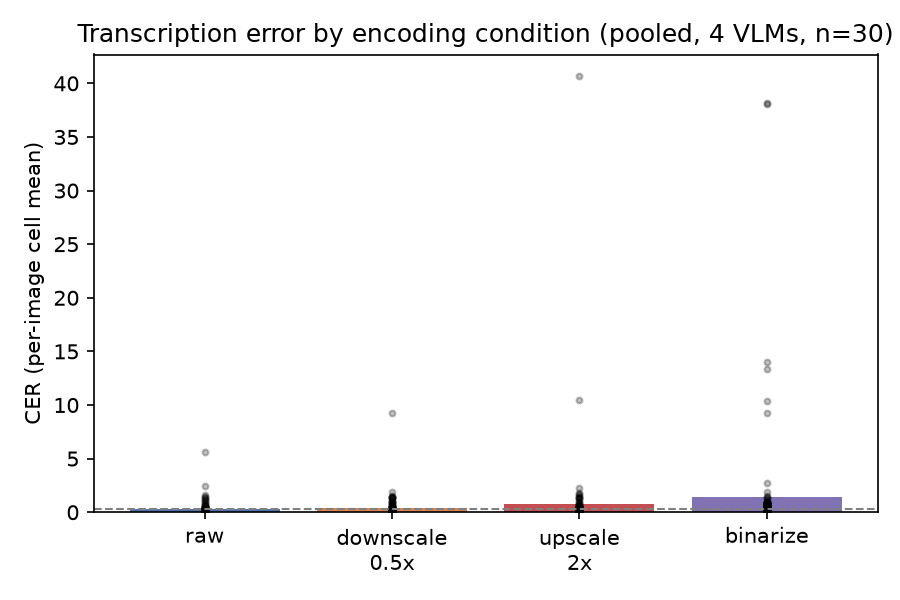
\includegraphics[width=0.62\textwidth]{figures/fig_cer_by_condition.png}
\caption{Character error rate by encoding condition, pooled across four vision-language models, with
per-image cell means overlaid as points and the raw baseline marked by the dashed line. Error rises
monotonically from raw through downscale and upscale to binarization.}
\label{fig:cer}
\end{figure}

\paragraph{The raw image is the best input.}
Across the four models the raw condition records the lowest error on both metrics, at 0.297 for
character error rate and 0.457 for word error rate, and error grows monotonically through the
downscale, upscale, and binarization conditions. Because the reconstructed ground truth omits
header and footer text, these absolute levels are inflated upper bounds rather than literal
recognition rates, and the inferential weight rests on the paired differences reported next, which
difference out a per-image offset that is approximately constant across conditions.

\paragraph{Paired contrasts confirm that encoding hurts.}
Table~\ref{tab:contrasts} reports the paired difference of each encoding against the raw image.
Two of the three encodings raise error with bootstrap intervals excluding zero on both metrics.
Upscaling raises character error rate by 0.431 (interval 0.077 to 1.631, $d_z = 0.257$, Wilcoxon
$p = 0.023$), a result that runs against the prior expectation that enlargement would help, and
binarization raises it by 1.163 (interval 0.512 to 2.390, $d_z = 0.468$, Wilcoxon $p = 0.004$).
Downscaling is directionally harmful but its pooled interval includes zero (difference 0.078,
interval $-0.031$ to 0.383, $p = 0.191$). The independent percentile bootstrap agrees with the
accelerated bootstrap in sign and in bracketing of zero for all three contrasts, and the
independently recomputed mean differences and effect sizes match the pipeline exactly.

\begin{table}[h]
\centering
\caption{Paired contrasts of each encoding against the raw image, pooled over the four models, on
$n = 30$ images. The difference is condition minus raw, so a positive value denotes higher error.
Intervals are bias-corrected and accelerated bootstrap at ninety-five percent; the Wilcoxon column
is exploratory.}
\label{tab:contrasts}
\begin{tabular}{llcccc}
\toprule
Metric & Contrast & Mean diff. & 95\% CI & $d_z$ & Wilcoxon $p$ \\
\midrule
CER & downscale $-$ raw & $+0.078$ & $[-0.031,\ 0.383]$ & 0.163 & 0.191 \\
CER & upscale $-$ raw   & $+0.431$ & $[\phantom{-}0.077,\ 1.631]$ & 0.257 & 0.023 \\
CER & binarize $-$ raw  & $+1.163$ & $[\phantom{-}0.512,\ 2.390]$ & 0.468 & 0.004 \\
\midrule
WER & downscale $-$ raw & $+0.044$ & $[-0.205,\ 0.286]$ & 0.065 & 0.084 \\
WER & upscale $-$ raw   & $+1.042$ & $[\phantom{-}0.055,\ 4.406]$ & 0.233 & 0.031 \\
WER & binarize $-$ raw  & $+2.467$ & $[\phantom{-}0.723,\ 6.442]$ & 0.353 & 0.002 \\
\bottomrule
\end{tabular}
\end{table}

\paragraph{The harm generalizes across models.}
Every one of the twelve model-by-condition contrasts carries a positive sign, so each encoding
raised character error rate for each model, a uniformity displayed per model in
Figure~\ref{fig:forest}. Binarization is the most consistent harm across the set, surviving the
Holm correction for the Google model and remaining the largest mean shift for the others, while the
upscale harm concentrates in the OpenAI and Mistral models and the downscale effect stays small
throughout. Mistral records the largest mean shifts together with non-significant rank tests, a
pattern produced by a small number of catastrophic items inflating the mean while the median shift
stays modest, which is the heavy-tailed case in which the rank test and the mean diverge and a
reason to report both.

\begin{figure}[h]
\centering
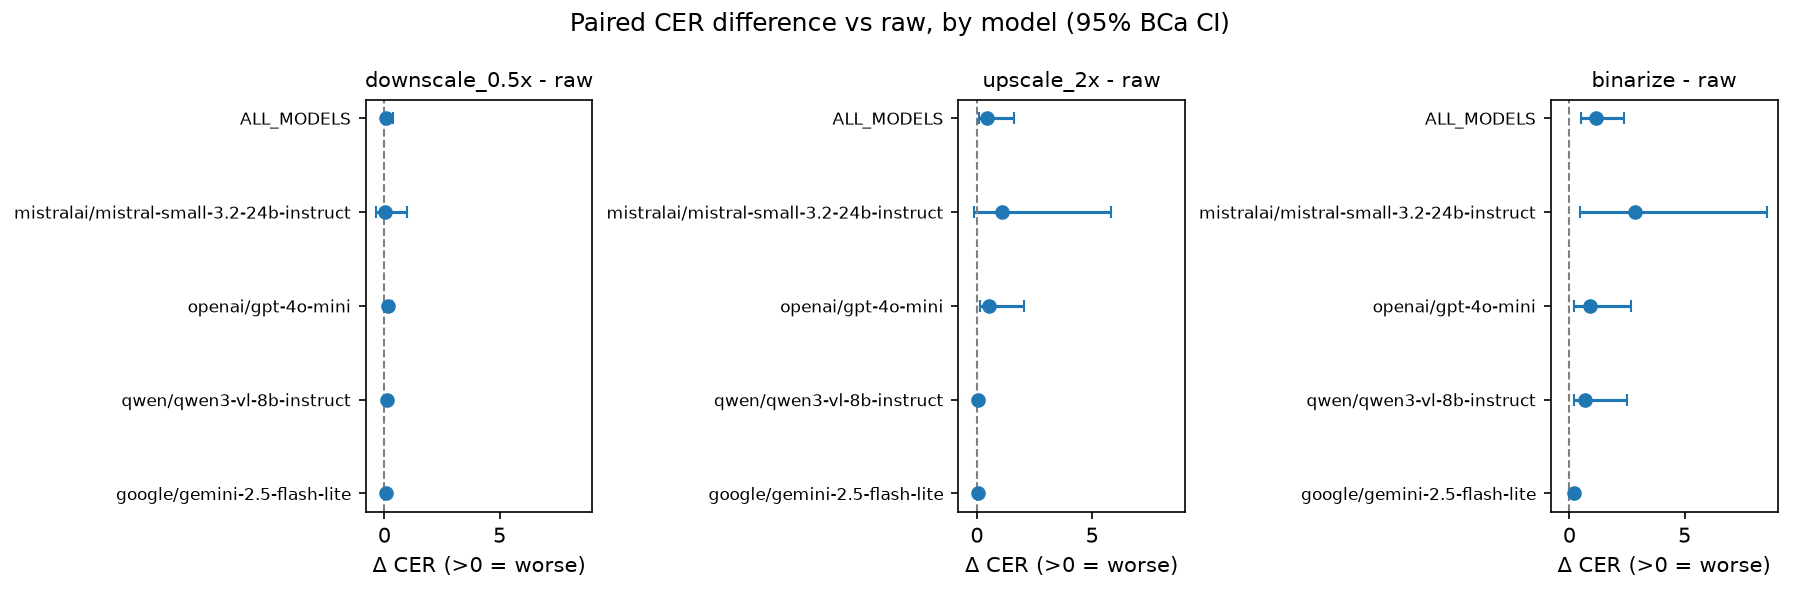
\includegraphics[width=0.95\textwidth]{figures/forest_cer.png}
\caption{Per-model paired difference in character error rate for each encoding relative to the raw
image, with ninety-five percent bootstrap intervals. Points to the right of the dashed zero line
denote higher error than raw. All points lie to the right.}
\label{fig:forest}
\end{figure}

\paragraph{Degradation amplifies non-determinism.}
The raw condition is close to reproducible across the three identical temperature-zero calls, with a
mean within-cell character-error standard deviation of 0.051, whereas degradation raises that
instability by one to two orders of magnitude, reaching 0.434 under upscaling and 1.060 under
binarization, the latter exceeding the mean effect itself (Figure~\ref{fig:nd}). Hosted-model
non-determinism is therefore not a constant background, but an input-dependent quantity that
explodes when the image becomes ambiguous, so that a single deterministic pass on a degraded input
reports one draw from a wide distribution.

\begin{figure}[h]
\centering
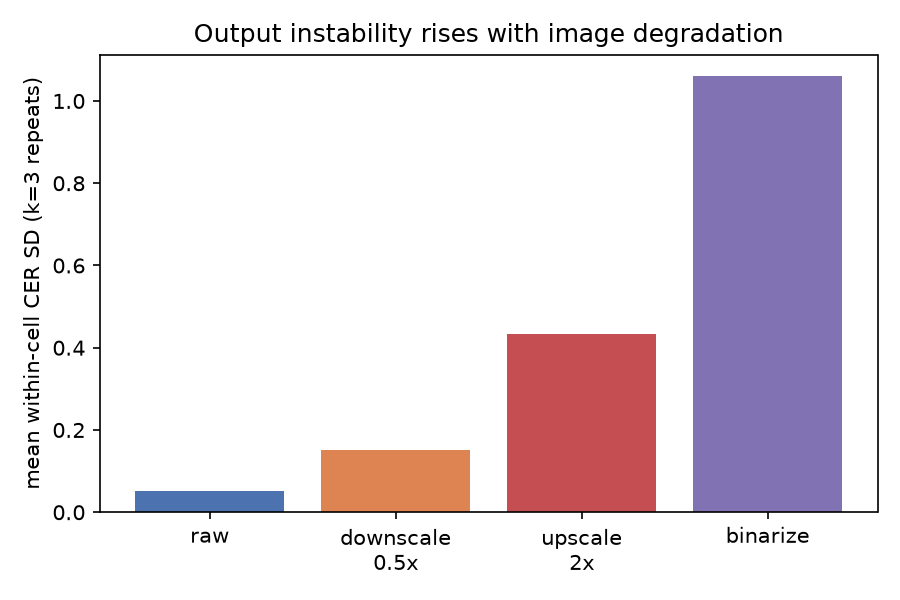
\includegraphics[width=0.62\textwidth]{figures/fig_nondeterminism.png}
\caption{Mean within-cell standard deviation of character error rate across the three repeated calls,
by condition. Output instability rises sharply as the image is degraded.}
\label{fig:nd}
\end{figure}

\paragraph{Mechanism and robustness.}
Inspection of output length indicates the route by which degradation produces error. The Mistral and
OpenAI models emit substantially more text under binarization and upscaling, against a gold mean of
118 characters their binarized outputs reach 357 and 256 characters respectively, consistent with
hallucinated or misread content entering as insertions, whereas the Google model emits less under
binarization, consistent with dropped content entering as deletions. Both routes raise edit
distance. The condition ordering, raw below downscale below upscale below binarize, holds identically
under all three normalization variants, so the conclusion does not depend on the punctuation or
case decisions in the scoring pipeline.

\paragraph{Structured fields confirm the ranking without the coverage confound.}
Scoring against the corpus structured parse, which checks only specific gold amounts and is therefore
immune to header coverage, reproduces the edit-distance ranking and sharpens it (Table~\ref{tab:field}
and Figure~\ref{fig:field}). Binarization collapses field recall from 0.945 to 0.667 and the
total-hit rate from 0.964 to 0.656, with paired differences of $-0.278$ (interval $-0.432$ to
$-0.145$, $p = 0.002$) and $-0.308$ (interval $-0.479$ to $-0.164$, $p = 0.002$). Upscaling lowers
field recall by 0.033 ($p = 0.023$). Downscaling, against its small edit-distance cost, leaves field
accuracy unchanged ($+0.009$, $p = 0.666$), which indicates that the downscale signal in the
edit-distance metric was largely header and formatting noise that the field metric removes. The two
ground-truth constructions agree on the ranking and on the two significant harms, providing the
strongest internal-consistency evidence the pilot affords.

\begin{table}[h]
\centering
\caption{Structured field accuracy by encoding condition, scored against the CORD structured parse
(higher is better, immune to the header-coverage confound). Field recall is the fraction of gold
amounts present; total hit is the receipt-total transcription rate.}
\label{tab:field}
\begin{tabular}{lcc}
\toprule
Condition & Field recall & Total-hit rate \\
\midrule
raw            & \textbf{0.945} & \textbf{0.964} \\
downscale 0.5$\times$ & 0.954 & 0.967 \\
upscale 2$\times$     & 0.913 & 0.939 \\
binarize       & 0.667 & 0.656 \\
\bottomrule
\end{tabular}
\end{table}

\begin{figure}[h]
\centering
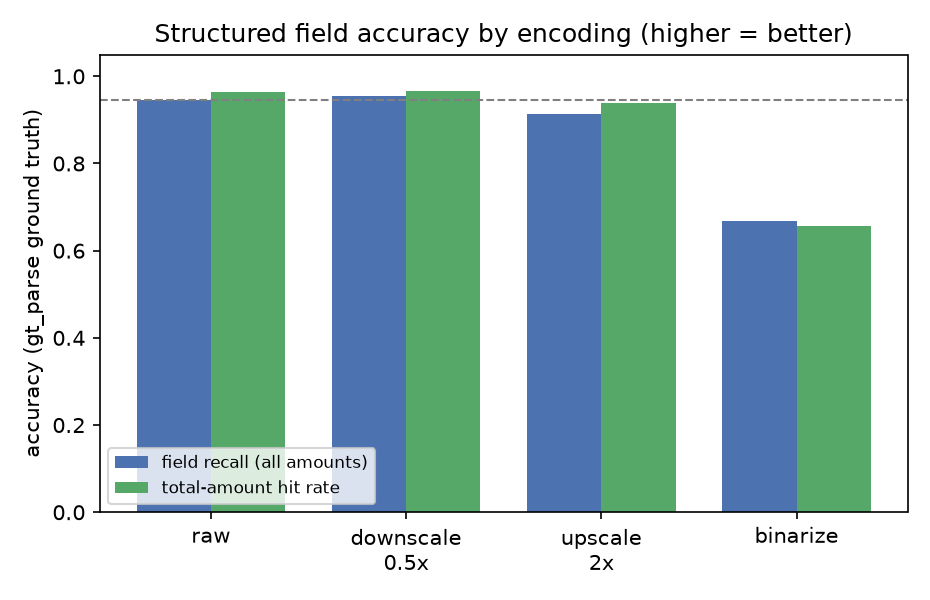
\includegraphics[width=0.62\textwidth]{figures/fig_field_accuracy.png}
\caption{Structured field accuracy by encoding condition, scored against the CORD structured parse.
Binarization collapses both the fraction of gold amounts recovered and the total-transcription rate,
while downscaling matches the raw baseline.}
\label{fig:field}
\end{figure}

\paragraph{The judge calibrates at human level without human labels.}
Calibrated against the deterministic field oracle on forty balanced pairs, the judge reached 85.0
percent agreement and a Cohen's kappa of 0.70, a substantial level that clears the pre-set
admissibility threshold of 0.61 and matches the human-level agreement reported for strong judges
\citep{zheng2023judge}. The calibration is reported as agreement with an objective oracle rather than
with a human adjudicator.

\section{Discussion}

The central finding inverts a long-standing default. For receipts already legible to a human reader,
the unaltered image is the strongest input to a vision-language transcriber, and the standard
cleanup operations of classical recognition degrade rather than improve the result. Binarization
proceeds as the clearest case, and its harm admits a direct mechanism, since a global Otsu threshold
applied to a photographed thermal receipt, carrying shadows, gradients, and faint low-contrast
print, fragments or erases glyphs that the model would otherwise read, after which the model either
fabricates replacement text or drops the line.

The refutation of the upscaling prediction is the most instructive negative result. Super-resolution
assists recognition when the text is too small to resolve \citep{wang2020textzoom}, a condition that
the CORD receipts do not satisfy at native resolution, so two-times enlargement supplies no
legibility that was missing and instead enlarges the surface on which the weaker models fail. The
actionable reading is conditional rather than blanket, namely that a resolution intervention should
be expected to help only where measured input resolution sits below the legibility threshold, and
not as an unconditional encoding step.

The original motivation envisioned a sellable encoder whose transform improves downstream accuracy,
and the honest implication of these results reshapes that proposition. For legible documents the
highest-return encoder is a pass-through, a tool defaulting to binarization would actively reduce
accuracy, and any defensible value proposition rests on a gating policy that intervenes only when a
resolution measurement warrants it. The non-determinism result carries a second implication for
evaluation practice, since any benchmark that scores degraded inputs through a single hosted call is
reporting an unstable draw, and repeated sampling with reported variance becomes necessary precisely
in the conditions where models are stressed.

\section{Limitations}
\label{sec:limitations}

Several constraints bound these conclusions, and each maps to a specific extension. The reconstructed
ground truth covers itemized fields and omits header and footer text, so the absolute error levels
are inflated and only the paired contrasts are interpreted, with the residual risk being an
interaction in which binarization drops the faint header and thereby lowers the insertion penalty, a
bias that would work against the binarization finding and therefore renders the reported harm a
conservative estimate. The sample is small and single-domain, thirty receipts in printed Latin
script, so no claim extends to handwriting, scene text, dense multi-column documents, or non-Latin
scripts, and the study is framed as a feasibility and estimation pilot rather than a powered
confirmatory test, with the reported $p$-values treated as exploratory \citep{leon2011pilot}.
Several intervals are wide because catastrophic failures generate heavy tails, so the rank tests and
medians deserve more trust than the means in those cells. Provider behavior is partly opaque, since
the two-times upscale produced large images and server-side resizing is undocumented, leaving the
upscale effect partly unattributable. The semantic-equivalence judge was calibrated against a
deterministic structured-gold oracle rather than human labels, an objective reference that certifies
content equivalence rather than the full semantic nuance a human adjudicator would supply, and no
judge-adjusted error quantities are reported beyond the calibration agreement itself.

A fuller study follows directly from these constraints. Obtaining full-page ground truth would make
absolute error meaningful and remove the coverage confound, additional regimes would test
generalization and would furnish the low-resolution inputs under which the super-resolution
prediction should finally hold, a mixed-effects specification with image and model as random effects
would use the data more efficiently than the collapse-then-pair analysis and would model the
variance structure that the non-determinism result exposed, and a denser resolution sweep would map
the dose-response curve and locate the legibility threshold that the conditional-encoder policy
requires.

\section{Conclusion}

In summary, our results provide a consistent narrative across 1{,}440 transcriptions of thirty
receipts by four vision-language models. The raw image should be the default input, with downscaling
mildly degrading accuracy, two-times upscaling degrading it further, and Otsu binarization degrading
it most, and with the ordering holding for every model and every normalization variant. Image
degradation additionally amplifies run-to-run instability, showing hosted-model non-determinism to
be input-dependent rather than constant. The classical reflex to binarize and normalize before
recognition is counterproductive for legible documents read by these models, and the appropriate
preprocessing default is to leave a readable image alone and to intervene only when measured
resolution is too low to read. Every quantity in this report was confirmed through an independent
re-derivation, and the dataset sample, model outputs, scores, and analysis code will be released
in a public repository to support reproduction.

\section*{Acknowledgments}

This study began as a live demonstration for Eric Kwon of what an AI-orchestrated research
pipeline can produce in a single working session, and the author credits him for prompting
the question it answers.

\bibliographystyle{plainnat}
\bibliography{references}

\end{document}
